\chapter{Analyse}\label{ch:analyse}

Bevor auf Grundlage der architekturellen Ideen aus \Cref{ch:grundlagen} ein konkretes Lösungskonzept entwickelt werden konnte, musste die bestehende App zunächst analysiert werden. Diese auf den Entwicklungsprozess vorbereitenden, analytischen Aspekte sollen in diesem Kapitel erörtert werden, um im nächsten Kapitel die konkreten Implementationskonzepte vorzustellen.

\section{Ermittlung einer Dialoglandkarte}

Zu Beginn der Analyse wurde die bestehende iOS App getestet, um alle möglichen Navigationswege und Dialoge zu sammeln und innerhalb einer Übersicht zu betrachten.

\begin{figure}[H]
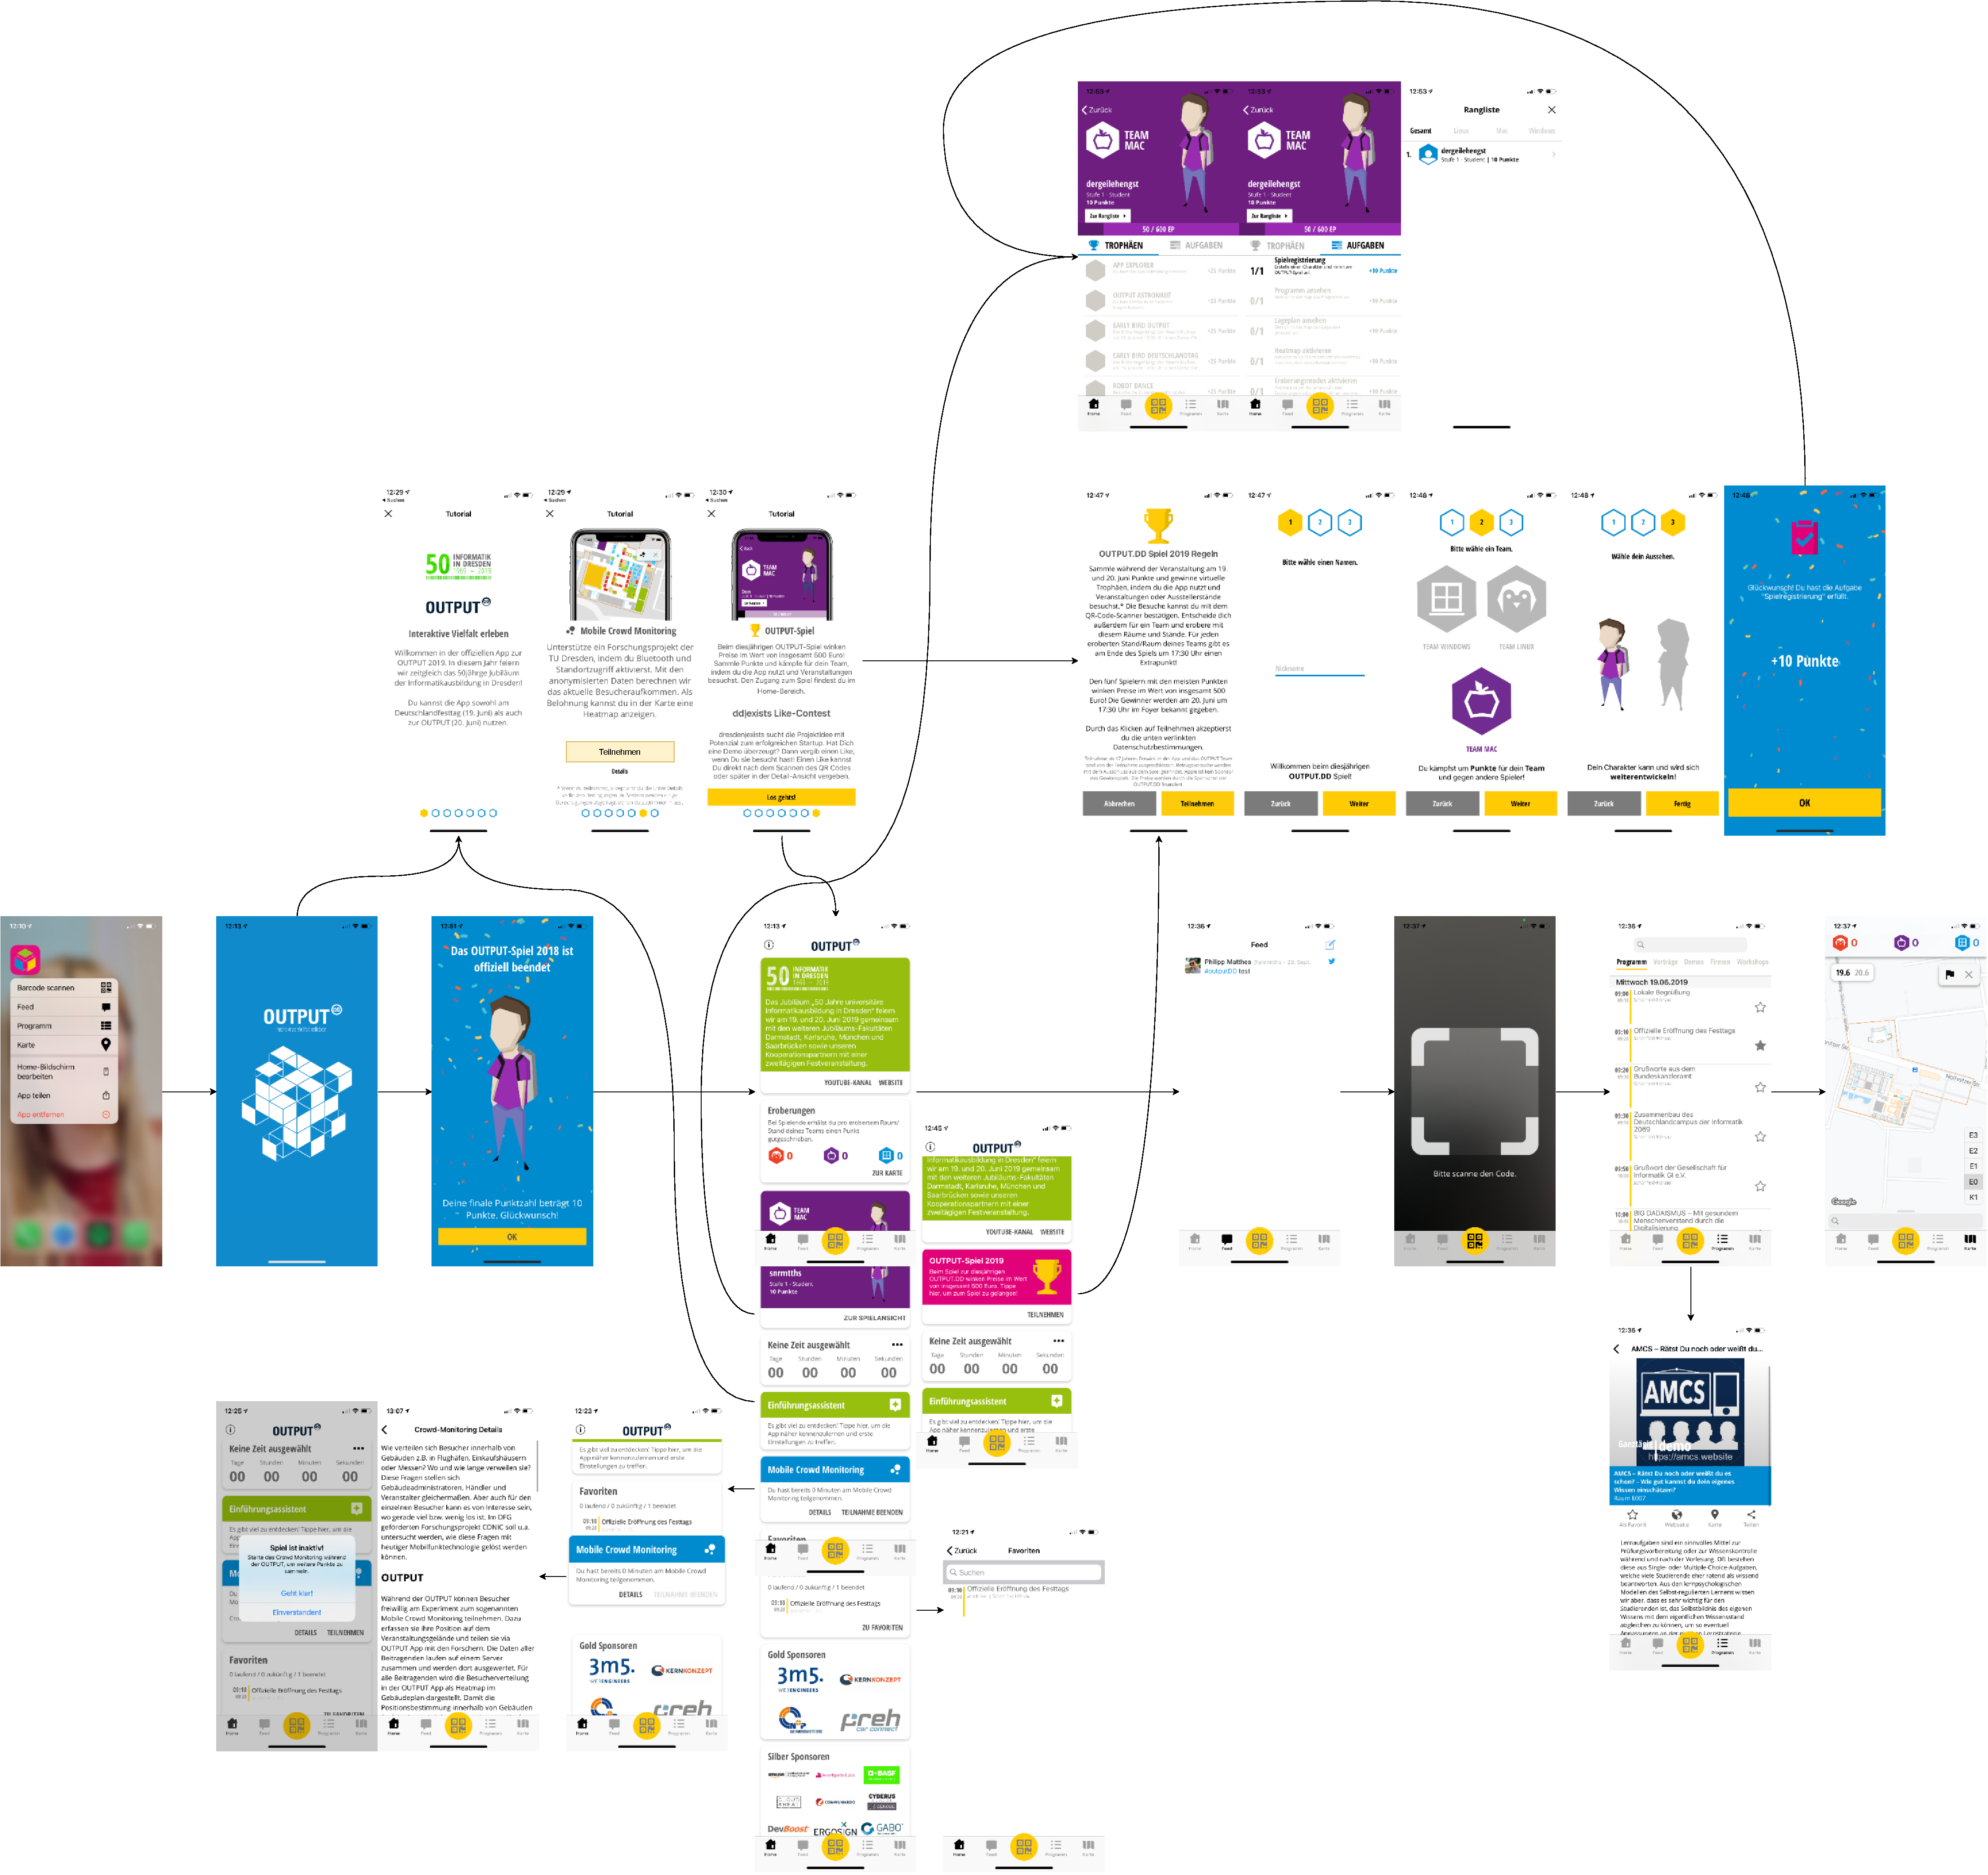
\includegraphics[width=\linewidth, bb=0 0 2123 2002]{mindmap.pdf}
\caption{Die erstellte Dialoglandkarte zur bestehenden Version der iOS App zeigt die Navigationswege innerhalb der App, sowie die genutzten UI-Elemente.}\label{fig:swiftui}
\end{figure}

Die in \Cref{fig:swiftui} gezeigte Dialoglandkarte suggeriert bereits die verschiedenen Gruppierungen von Ansichten, welche wir später zur Erstellung von neuen Packages heranziehen konnten. Zu sehen ist beispielsweise, dass die Spiel-Ansichten, der Einführungsassistent, oder bspw. auch die Kalender-Ansicht bereits gut voneinander separierbar sind. Die aufgezeichneten Navigationspfeile zwischen den Ansichten konnten genutzt werden, um die Datenflüsse hierbei vor der Erstellung des Konzeptes besser zu verstehen und die jeweils hierfür am Besten geeigneten Patterns zu finden.

\section{Struktur des Couchbase-Datenbank-Frameworks}



